\documentclass[sigconf,anonymous]{aamas}
\usepackage{amsmath}
\usepackage{algorithm}
\usepackage{algpseudocode}
\usepackage{tikz}
\usetikzlibrary{arrows.meta,positioning}
% Copyright and conference block copied from the official AAMAS 2027 sample.
\makeatletter
\gdef\@copyrightpermission{
  \begin{minipage}{0.2\columnwidth}
   \href{https://creativecommons.org/licenses/by/4.0/}{
\includegraphics[width=0.90\textwidth]{by}}
  \end{minipage}\hfill
  \begin{minipage}{0.8\columnwidth}
   \href{https://creativecommons.org/licenses/by/4.0/}{This work is licensed under a Creative Commons Attribution International 4.0 License.}
  \end{minipage}
  \vspace{5pt}
}
\makeatother
\setcopyright{ifaamas}
\acmConference[AAMAS 2027]{Proc.\@ of the 26th International Conference
on Autonomous Agents and Multiagent Systems (AAMAS 2027)}{3--7 May 2027}{Hanoi, Vietnam}{M.~Baldoni, F.~Fang, W.~Yeoh, N.~Yorke-Smith (eds.)}
\copyrightyear{2027}
\acmYear{2027}
\acmDOI{}
\acmISBN{}
\acmSubmissionID{INTERNAL REVISION}
\submissionType{Research Paper Track}


\title[When Should an Agent Earn Delegation?]{When Should an Agent Earn Delegation? Evidence, Reputation, and Coordination in Language-Agent Teams}
\ccsdesc[500]{Computing methodologies~Multi-agent systems}
\keywords{Multiagent coordination, delegation, reputation, language agents, budgeted evaluation}

\begin{abstract}
Delegating a task requires deciding whose previous work deserves trust. In language-agent teams, a high acceptance rate can reflect useful competence, a permissive auditor, or repeated exposure to easy tasks. We study evidence-derived organization through this distinction between accepted work and demonstrated delegation value. We specify a local protocol in which task-conditioned interaction records change future executor selection, and analyze when noisy acceptance preserves competence rankings. The analysis shows that informative, worker-independent audits preserve expected rankings, whereas fixed-step updates retain uncertainty and cannot guarantee converged roles. We also reanalyze existing small-model question-answering results to identify what they establish: dataset-specific adaptive routers improve answer F1, most substantially on 2Wiki, but their scores do not identify a benefit from persistent reputation. Neutral selector interventions, missing complete cost records, and a concrete failed audit trace delimit the current evidence. This distinction yields falsifiable tests of organization: preserve tools and budgets while freezing, shuffling, or transferring the state used for delegation. Evidence should earn routing authority only when its contribution survives these controls.
\end{abstract}

\begin{document}
\maketitle

\noindent\textbf{Internal revision status.} The protocol and prospective tests in Sections~\ref{sec:protocol} and~\ref{sec:tests} are a revised research design. Section~\ref{sec:results} reports reanalysis of preserved experiments, not measurements of that revised protocol. New protocol experiments must be completed before submission.

\section{Introduction}

Language-agent teams need to decide who should act, who should check an answer, and when another interaction is worth its cost. Fixed role prompts provide a convenient initial assignment, but they do not establish that a particular worker has earned future responsibility. Conversely, replacing fixed roles with a dynamic router does not establish that the router learns from its workers. It may simply select a useful prompt or tool from the current question.

The distinction matters because organization is a property of interactions over time. A team becomes organized through evidence only if previous contributions change subsequent allocation, and those changes improve coordination. Partner-selection research already treats interaction history as a determinant of later cooperation~\cite{leung2025partner,russell2026partner}. Reputation mechanisms similarly connect observed behavior to future relationships~\cite{ren2026reputation}. For language-agent reasoning, the unresolved question is more specific: \emph{when does an upstream agent's acceptance of a contribution justify giving that worker more responsibility?}

Acceptance is an imperfect observation. An auditor can endorse an unsupported answer; a worker can succeed on easy tasks while avoiding difficult ones; a useful intermediate contribution can occur inside a failed episode. Updating a worker's reputation from these events can amplify either competence or error. A system that logs audit labels without enforcing their consequences may also appear more structured than its execution actually is. These possibilities make answer accuracy an insufficient measure of organizational learning.

We retain the principle of \textbf{Evidence-Derived Organization (EDO)} but give it a narrower operational meaning: accepted, attributable contributions update local, task-conditioned estimates that influence future delegation. The research object is the relationship between evidence, allocation, and team utility. Task trees, memory, and tools are supporting mechanisms whose independent effects must be controlled, not interchangeable evidence that organization has emerged.

This paper develops three connected objects. First, a local delegation protocol separates evidence retrieval from reputation used for executor selection. Second, an elementary analysis relates auditor error to the reliability of competence estimates and corrects the convergence interpretation of constant-step updates. Third, a reanalysis of existing question-answering experiments distinguishes measured router performance from untested persistent organization. Together they define a testable account of earning responsibility, rather than treating a performance improvement as proof of emergent roles.

The empirical starting point is useful but limited. Preserved Qwen2.5-3B experiments report F1 gains of 0.0045, 0.0130, and 0.0857 over the selected strongest comparison rows on HotpotQA, MuSiQue, and 2Wiki. These are three dataset-specific implementations. Their current runner does not preserve learned reputation across examples. We therefore use these results to motivate the revised tests, and do not attribute them to persistent specialization.

\section{Related Work}

\paragraph{Partner selection.}
Leung et al.~\cite{leung2025partner} study experience-dependent partner selection and the resulting interaction networks in language games. Russell et al.~\cite{russell2026partner} investigate partner selection when agents initially lack information about each other. Albers et al.~\cite{albers2024roles} measure roles through interaction structure in an agent-based market. These studies motivate measuring who works with whom, how that changes, and what the change explains. They do not imply that any specialization statistic establishes useful reasoning roles.

\paragraph{Reputation and adaptive language-agent systems.}
RepuNet~\cite{ren2026reputation} combines reputation with evolving relationships to sustain cooperation in language-agent societies. AgentNet~\cite{yang2025agentnet} already studies decentralized routing, evolving connections, and specialization. Consequently, neither decentralization nor history-dependent organization alone is a novelty claim for EDO. The proposed distinction is the use of attributable, task-conditioned acceptance records for budgeted delegation, together with explicit tests that remove or corrupt those records while holding the execution machinery fixed.

\paragraph{Dynamic roles and workflow optimization.}
Dynamic Role Assignment~\cite{zhang2026dynamic} selects candidates through proposals and peer review before debate. GPTSwarm~\cite{zhuge2024gptswarm} optimizes language-agent graphs, while MoRSE~\cite{li2026morse} studies role--subtask specialization with parameter adaptation. These are closer conceptual alternatives than a large list of general orchestration libraries. EDO's proposed online, local state update must therefore be compared against capability-aware selection and a simple history-based bandit, not only against fixed prompts. The bandit comparison follows the established distinction between observing rewards and allocating exploration~\cite{auer2002finite}.

\paragraph{Trees, memory, and retrieval.}
ReAcTree~\cite{choi2026reactree} combines a dynamic agent tree, control flow, and memory for long-horizon planning. SCMRAG~\cite{agrawal2025scmrag} uses self-correction in multihop retrieval. These works preclude attributing novelty to the presence of a task tree, a memory store, or corrective retrieval alone. Our proposed experiment isolates executor-selection state from reusable context, tool availability, and current-answer revision.

\section{A Protocol for Earning Delegation}
\label{sec:protocol}

The protocol produces an answer, a resource ledger, and an auditable record of which accepted contributions affected later allocation. It uses a fixed local communication graph and a shared model and tool interface. Persisting the allocation state across tasks is an explicit part of the revised design; it is not inferred from the historical experiments.

\subsection{Task and information boundary}

Let $G=(\mathcal A,\mathcal E)$ be a directed graph of agents. For agent $i$, $\mathcal N(i)$ is the set of neighbors to which it may delegate. An input $x_t=(q_t,C_t)$ contains a task and its available context. A gold answer, hidden test, or other evaluation label is held outside the policy and is used only for scoring. The decision state contains the current task, the agent's local records, and summaries directly received from neighbors. It excludes a global worker-ranking table.

A task node $z$ specifies a requested output, evidence references, an owner, and a remaining budget. Its type $k(z)$ comes from a task taxonomy frozen before evaluation. For the first implementation, use a small set of observable demands such as extraction, comparison, and composition; no benchmark name or gold-label-derived feature may select a policy. Task type is an input descriptor, not an agent identity.

Agent $i$ keeps two separate stores. Its task memory $M_i$ contains retrievable observations and intermediate outputs. Its allocation record contains an estimate $r_{ij,k}\in[0,1]$ and count $n_{ij,k}$ for each neighbor $j$ and task type $k$. The estimate summarizes acceptance outcomes on tasks actually assigned by $i$ to $j$. Keeping the stores separate allows an experiment to preserve all task evidence while removing reputation.

\subsection{Delegate, verify, and record}

At each decision, an agent can solve locally, delegate to a neighbor, or split a composite task into bounded subtasks. For a delegated subtask, the executor returns a candidate output together with references to the evidence used. The owner checks output validity, evidence support, and subtask completion before integration. An audit can accept, request a revision, reroute, or resplit. A non-acceptance action must change execution or terminate the task; writing a label alone does not satisfy the protocol.

For each audited delegation, let $A_{ij,k}\in\{0,1\}$ indicate whether the returned contribution was accepted. The record includes the task type, executor, audit outcome, cited evidence, actual cost, and the resulting control action. Acceptance is an observation of the owner, not an oracle correctness label. Rejected attempts remain in the record and affect the acceptance estimate; otherwise the estimate would condition on success and reward selective omission.

For a chosen update rate $0<\mu\leq1$, update the selected edge and task type:
\begin{equation}
 r_{ij,k}^{+}=(1-\mu)r_{ij,k}+\mu A_{ij,k},
 \qquad n_{ij,k}^{+}=n_{ij,k}+1.
 \label{eq:update}
\end{equation}
Unobserved edges are not updated. The event advances the persistent allocation state only after its audit has completed. Current-task evidence may still be integrated during execution, but future tasks cannot observe an unfinished outcome.

The minimal policy chooses a feasible neighbor using estimated acceptance minus predicted cost:
\begin{equation}
 j^*\in\arg\max_{j\in\mathcal N(i)}
 \{r_{ij,k(z)}-\lambda\widehat c_{ij,k(z)}\}.
 \label{eq:route}
\end{equation}
A fixed exploration probability selects a feasible neighbor uniformly; otherwise the policy uses Equation~\eqref{eq:route}. This makes the opportunity to acquire evidence explicit. Initial estimates and prompts are identical across workers. Graph position and prior interactions may create asymmetry, but predefined specialist names must not do so. The cost weight, update rate, and exploration probability are selected on development tasks and frozen before evaluation. A cost-aware contextual bandit using the same observations is a required alternative, since a moving average is not itself a new learning algorithm.

\begin{figure}[t]
\centering
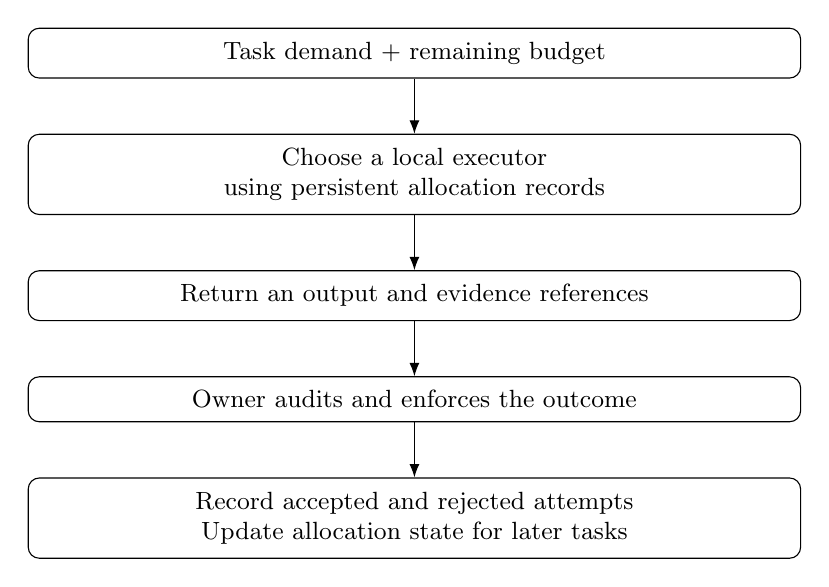
\begin{tikzpicture}[node distance=7mm,>=Latex,every node/.style={font=\small},box/.style={draw,rounded corners,align=center,text width=0.78\columnwidth,inner sep=5pt}]
\node[box] (task) {Task demand + remaining budget};
\node[box,below=of task] (select) {Choose a local executor\\using persistent allocation records};
\node[box,below=of select] (work) {Return an output and evidence references};
\node[box,below=of work] (audit) {Owner audits and enforces the outcome};
\node[box,below=of audit] (record) {Record accepted and rejected attempts\\Update allocation state for later tasks};
\draw[->] (task)--(select);
\draw[->] (select)--(work);
\draw[->] (work)--(audit);
\draw[->] (audit)--(record);
\end{tikzpicture}
\caption{Revised protocol. Task memory supplies evidence; allocation records change who receives later work. Freezing the latter preserves the former. This diagram specifies the proposed design, not a claim that historical routers implement persistent state.}
\Description{Five sequential steps: receive task demand and budget, choose a local executor using persistent records, return output and evidence, audit and enforce the result, and update future allocation records.}
\label{fig:protocol}
\end{figure}

\subsection{Budget enforcement and locality}

Every model invocation, including decomposition, auditing, integration, and retries, acquires a reservation from the same episode budget before dispatch. A call limit $B$ bounds attempted invocations, not the number of visible handoffs. A token limit separately accounts for prompt and completion tokens; a request reserves its prompt length and maximum output length and releases unused capacity on return. The driver records exceptions and requests with missing usage fields instead of silently treating them as free. Deterministic tool time and parallel wall-clock are reported separately.

The call-count guarantee is an implementation invariant: if the counter starts at zero and a request is issued only after an atomic increment that keeps it at most $B$, there can be at most $B$ issued requests. This replaces a bound inferred from tree depth whose validity depends on how retries and audits are implemented. Locality likewise requires checking the fields consumed by the router, not simply storing a sparse adjacency list.

\begin{algorithm}[t]
\caption{Evidence-derived delegation: proposed execution contract}
\label{alg:delegation}
\begin{algorithmic}[1]
\Require Ordered tasks; graph; persistent records; frozen budget
\For{each task $x_t$}
  \State Initialize task memory and an episode resource ledger
  \While{unresolved work and a feasible budget reservation}
    \State Read local demand and available neighbor records
    \State Select solve, delegate, or bounded split
    \State Reserve resources before every model request
    \State Obtain candidate output and evidence references
    \State Owner audits the delegated contribution
    \State Enforce accept, revise, reroute, or resplit
    \State Append outcome, attribution, and usage records
    \State Update the observed edge using Eq.~\eqref{eq:update}
  \EndWhile
  \State Return answer or explicit budget exhaustion
  \State Score externally; do not expose held-out labels to policy
\EndFor
\end{algorithmic}
\end{algorithm}

\section{What Acceptance Can Identify}
\label{sec:analysis}

The analysis concerns one task type and a fixed worker under an explicit observation model. It does not establish convergence or regret guarantees for the adaptive, heterogeneous team. Its purpose is to identify the audit quality that the experiments must measure.

Let $Y\in\{0,1\}$ denote whether a contribution is correct, with worker competence $p=\Pr(Y=1)$. Let $A$ be the audit's acceptance decision, with false-acceptance rate $\alpha=\Pr(A=1\mid Y=0)$ and false-rejection rate $\beta=\Pr(A=0\mid Y=1)$. Assume these rates are stationary and the same across the workers being compared within this task type.

\begin{proposition}[Acceptance preserves rankings conditionally]
The expected acceptance rate is
\begin{equation}
 q=\mathbb E[A]=\alpha+(1-\alpha-\beta)p.
 \label{eq:audit}
\end{equation}
It preserves strict competence order exactly when $\alpha+\beta<1$. At equality it contains no competence-ranking signal; above one it reverses the order.
\end{proposition}
\begin{proof}
Conditioning on correctness gives $q=\alpha(1-p)+(1-\beta)p$. For two workers, subtracting their expectations gives $(1-\alpha-\beta)(p_1-p_2)$, which has the asserted sign.
\end{proof}

This condition is not sufficient when the auditor treats workers differently or when task difficulty differs across their assigned samples. For example, a worker with $p_1=0.8$, $\alpha_1=0$, $\beta_1=0.5$ has $q_1=0.4$, while a weaker worker with $p_2=0.6$, $\alpha_2=0.5$, $\beta_2=0$ has $q_2=0.8$. Each auditor is individually informative, yet acceptance ranks the workers incorrectly. Reputation therefore needs conditional evaluation, controlled exposure, and auditor-error measurements.

\begin{proposition}[A fixed update rate retains uncertainty]
Suppose audited observations are independent Bernoulli variables with mean $q$, and the initial estimate $r_0$ is fixed. For Equation~\eqref{eq:update} after $n$ observations,
\begin{align}
 \mathbb E[r_n]&=q+(1-\mu)^n(r_0-q),\\
 \operatorname{Var}(r_n)&=\frac{\mu q(1-q)}{2-\mu}
 \left[1-(1-\mu)^{2n}\right].
 \label{eq:variance}
\end{align}
For $0<q<1$, the estimate does not converge in mean square to $q$ at a fixed positive update rate.
\end{proposition}
\begin{proof}
Unrolling the recursion yields $(1-\mu)^n r_0+\mu\sum_{s=1}^n(1-\mu)^{n-s}A_s$. Linearity gives the mean. Independence and the geometric sum of squared weights give the variance. Its positive limit precludes mean-square convergence to a constant.
\end{proof}

With constant steps, evidence-derived allocation tracks recent acceptance and retains noise. With decreasing steps, consistency requires additional stationarity and sampling assumptions. Neither case establishes stable specialization in a changing team. The audit-noise experiment should therefore measure whether inaccurate acceptance creates unjustified concentration of responsibility, while the worker-swap experiment should measure whether useful history is discarded or transferred appropriately.

\section{Reanalysis of Preserved Experiments}
\label{sec:results}

\subsection{Evaluation populations and method identity}

The preserved experiments use Qwen2.5-3B-Instruct at temperature zero with project implementations of answer F1 and exact match. We recomputed these scores from all 24,815 stored headline predictions and checked unique example identifiers. The confidence intervals below are the archived paired-bootstrap intervals. They describe uncertainty conditional on the selected configurations and examples; they do not account for repeated development on validation data or establish robustness across new model runs.

The project scorer is not exactly the official HotpotQA scorer: normalization order and special-answer handling differ. Applying the official answer-F1 function to the same HotpotQA router outputs changes six example scores and changes the aggregate from 0.432403 to 0.432275. Table~\ref{tab:headline} preserves the project-scored historical comparisons; official-scored differences require rescoring both sides.

HotpotQA~\cite{yang2018hotpotqa}, MuSiQue~\cite{trivedi2022musique}, and 2WikiMultiHopQA~\cite{ho20202wiki} are separate evaluation populations. The earlier HotpotQA F1 of 0.7641 came from a 200-example GPT-4.1-mini calibration run. It is not comparable to the 7,405-example Qwen result and is excluded from the main comparison. Baselines in Table~\ref{tab:headline} are the selected strongest recorded comparison rows, not claims about every available system.

\begin{table*}[t]
\centering
\begin{tabular}{llrrrr}
\toprule
Dataset & Selected comparator & Examples & Comparator F1 & Router F1 / EM & $\Delta$F1 [archived 95\% CI] \\
\midrule
HotpotQA & Direct single agent & 7,405 & 0.4279 & 0.4324 / 0.3255 & 0.0045 [0.0025, 0.0065] \\
MuSiQue & AgentVerse adaptation & 4,834 & 0.3259 & 0.3389 / 0.2424 & 0.0130 [0.0030, 0.0228] \\
2Wiki & Debate adaptation & 12,576 & 0.4689 & 0.5545 / 0.4965 & 0.0857 [0.0763, 0.0954] \\
\bottomrule
\end{tabular}
\caption{Historical answer-quality observations, not measurements of the revised protocol. Different datasets use different router configurations. The HotpotQA comparator's archived statistics were checked; its original raw prediction file is absent at the archived local path. The other two pairings were recomputed from local predictions.}
\label{tab:headline}
\end{table*}

The implementation identities matter. The historical scalar calibration variants retain scalar competence across examples. The historical task-tree and frame variants maintain task-local state. The headline adaptive routers select answer protocols through question cues, dataset-specific settings, and narrow tool rules; the current runner initializes fresh state for each example. Table~\ref{tab:variants} makes these differences explicit. A task-local audit may help an answer without producing a persistent role.

\begin{table}[t]
\centering
\begin{tabular}{p{0.29\columnwidth}p{0.60\columnwidth}}
\toprule
Variant & State and evidence interpretation \\
\midrule
Scalar calibration & Persistent scalar competence; historical calibration only. \\
Task-tree / frame & Task-local split, audit, memory, and tool machinery; component tests. \\
Adaptive routers & Dataset-specific protocol/tool choices; headline QA scores; no demonstrated cross-task reputation. \\
Revised EDO & Persistent, task-conditioned local acceptance records; experiments pending. \\
\bottomrule
\end{tabular}
\caption{Four distinct experimental objects. The first three contain measured historical variants; the last is the revised protocol.}
\label{tab:variants}
\end{table}

\subsection{Effects and resource accounting}

The largest observed gain is on 2Wiki, where narrow comparison and relation-handling tools plausibly matter. HotpotQA improves by about 0.45 F1 points on the 0--100 scale. Its router records 2,616.42 API tokens per example, versus 1,846.13 for direct answering: approximately 41.7\% more tokens. This is an accuracy--cost trade-off, not evidence of equal-compute superiority. Recorded tokens for the MuSiQue and 2Wiki routers are 4,380.14 and 2,747.77 per example. Complete attempted-call totals and elapsed times for these headline runs are not available in the inspected artifacts.

The old task-tree call cap and scalar-calibration call cap belong to different variants. Neither substitutes for measurements of the adaptive routers. Baseline elapsed times cannot be relabeled as EDO times. The task driver also reports outer handoffs, which do not count all nested model requests. We keep these measurements distinct rather than deriving missing cost fields from handoff counts.

\subsection{Component evidence includes neutral and harmful effects}

The 500-example HotpotQA frame comparison provides a different experimental object from the full-validation routers. Table~\ref{tab:components} retains all major directions of evidence. Memory removal is harmful in this configuration, but it changes information supplied to the model as well as the machinery around the task. It is therefore not a clean intervention on persistent reputation. Replacing the tag selector with all tools or random tools yields intervals spanning zero. These controls do not support a claim that the learned selector is necessary.

\begin{table}[t]
\centering
\begin{tabular}{lrr}
\toprule
Condition & F1 & Difference from full frame \\
\midrule
Full frame & 0.4853 & -- \\
Direct single agent & 0.4346 & $-0.0507$ \\
Task-tree control & 0.4154 & $-0.0699$ \\
No memory & 0.4073 & $-0.0781$ \\
Static tools & 0.3627 & $-0.1227$ \\
All tools & 0.4858 & $+0.0005$ (CI spans 0) \\
Random tools & 0.4863 & $+0.0010$ (CI spans 0) \\
No tool history & 0.4882 & $+0.0028$ (CI spans 0) \\
Split disabled & 0.4334 & $-0.0519$ \\
Active task-tree audit & 0.4073 & $-0.0781$ \\
\bottomrule
\end{tabular}
\caption{Historical Qwen component matrix, 500 matched examples. Full-frame differences are descriptive for distinct configurations, not automatically one-component causal effects. The active audit is also 0.0081 below its task-tree parent. Full archived intervals are in the supplement.}
\label{tab:components}
\end{table}

The recorded usage events make one resource confound visible: the full frame has 1,477 usage records across these 500 tasks, compared with 500 for direct answering. These are counts of recorded usage events, not a reconstruction of failed or unlogged attempts. Even this partial ledger makes it inappropriate to interpret the full-frame difference as a benefit at an equal call budget.

\subsection{A concrete audit failure}

A preserved HotpotQA example asks whether Scott Derrickson and Ed Wood had the same nationality. The available context identifies both as American. The frame first registers two subtasks and forwards to a second node. That node logs \texttt{REJECT\_REROUTE} for the prior contribution, retrieves a memory entry, and then chooses to answer locally. Its final answer is ``no'', while the stored gold answer is ``yes''. Three model-usage records are present.

This trace establishes neither that every audit fails nor that every reroute label is ignored. It demonstrates a specific gap between recording an audit and enforcing its meaning in control flow. It also shows why accepted answers cannot be equated with verified correctness. The revised protocol requires a direct test of every non-acceptance transition and separate measurements of audit false acceptance and false rejection.

\subsection{What is not established}

The evidence does not yet establish useful role formation across tasks, superiority to the nearest dynamic-organization methods, or a benefit at matched call and token budgets. A framework-family matrix provides breadth across adaptations but does not replace these tests. Three sampled slices are not three independent model reruns. Existing synthetic workflow checks and repeatedly revised coding diagnostics do not establish generalization to a fresh public non-QA task. Accordingly, these experiments support a constrained observation about historical routers and identify the next causal tests.

\section{Decisive Tests of Organization}
\label{sec:tests}

This section specifies prospective experiments. It contains no invented outcome values. The first requirement is a frozen implementation and disjoint development and evaluation data. Previously inspected validation examples remain development or historical-analysis data. The evaluation manifest must fix task IDs, task order, prompts, backbone, tool access, budgets, and failure handling before the first new run.

\paragraph{Does evidence change useful allocation?}
Run persistent EDO, frozen allocation records, records shuffled between workers within task type, and records reset after every task. Keep task memory, audit prompts, model, tools, and budgets identical. A useful organization effect requires a reproducible utility advantage for the correct history over these controls, accompanied by changed executor allocation. Report assignment distributions conditioned on task type and exposure. Entropy or role diversity alone is insufficient: specialization can be arbitrary and harmful.

\paragraph{Is the gain allocation or additional inference?}
Compare a direct agent with self-consistency or revise-and-check under the same call and token caps, a static team with the same tools, uniform delegation, a simple contextual-bandit router, and close external alternatives. Charge meta-debate, workflow search, calibration, failed calls, and tool execution to the appropriate development or deployment ledger. Report quality--cost curves over several frozen budgets. Do not select the strongest baseline independently for each test item using its true answer; such an oracle is an upper bound, not a deployable comparator.

\paragraph{Can the team recover from wrong evidence?}
Introduce controlled audit noise and swap worker capabilities after a fixed number of tasks. The prediction from Section~\ref{sec:analysis} concerns expected ranking only under its assumptions. Test where it breaks under worker-dependent audit error and changing task difficulty. Measure recovery delay, allocation to unreliable workers, and cumulative task utility. Separate synthetic tests of the observation model from language-model experiments.

\paragraph{Does the result survive a stronger backbone and another task?}
Retain the small-model setting for continuity and add one materially stronger available open-weight backbone. Evaluate one external, executable non-QA task with team coordination and independently checkable outcomes. ReAcTree's embodied planning setting is a relevant task family, subject to an adapter feasibility check. If only a coding benchmark is feasible, compare matched tests, tools, and budgets and restrict the conclusion to coding rather than general coordination. Choose the task for the scientific question, not for a favorable preliminary score.

\paragraph{Statistics and failure criteria.}
For persistent systems, task order and team history induce dependence. Use independently reset streams with fixed recorded order seeds and report stream-level uncertainty; itemwise bootstrap intervals alone are insufficient. Include at least five independent streams for the primary contrast, while acknowledging that a small number of streams may still yield wide intervals. Use development data to choose the number of tasks needed for a predeclared minimum effect. Publish all frozen primary contrasts, including zero and negative effects. If frozen or shuffled records match the full policy, withdraw the learned-organization claim. If equal-budget direct reasoning matches the team, report the boundary instead of redefining success after seeing results.

\section{Discussion and Limitations}

The proposed view separates three quantities: an answer's quality, a contribution's acceptance, and the value of assigning future work to its producer. Only the third makes reputation an organizational mechanism. A high answer score with task-local heuristics can be useful engineering, but it answers a different question from whether workers earn delegation through experience.

Our elementary propositions characterize a restricted observation model. They do not prove equilibrium roles, global convergence, robustness to strategic workers, or efficient exploration. The historical study uses small models and previously developed configurations; complete cost accounting, fresh evaluation, and external dynamic-selection comparisons remain open. The comparison of current source code with historical artifacts is also bounded by the availability of exact runtime snapshots. These limitations determine the experiments needed to turn the revised account into a validated algorithmic contribution.

AI assistance was used in revising the hypotheses, mathematical analysis, experimental design, and manuscript. The supplementary disclosure records its scope and the available tool/version information; authors must verify and finalize that record and all scientific claims before submission.

\section{Conclusion}

Accepted work can justify delegation only when acceptance is informative, attributable, and causally useful for subsequent allocation. Existing QA gains motivate this question but do not establish persistent roles. A convincing evaluation must intervene on the allocation state while preserving task evidence and resources. This makes both successful organization and its failure conditions observable.

\bibliographystyle{ACM-Reference-Format}
\bibliography{references}
\end{document}
